\documentclass[11pt]{article}
\usepackage[margin=1in]{geometry}
\usepackage{amsmath,amssymb}
\usepackage{booktabs}
\usepackage{graphicx}
\usepackage{hyperref}
\usepackage{xcolor}
\usepackage{microtype}
\usepackage{natbib}

\hypersetup{colorlinks=true, linkcolor=blue, citecolor=blue, urlcolor=blue}

\title{\textbf{RIFT: A Conflict Signature for Deception in Language Models}\\
\large Label-free identification of deceptive responses via residual rank ---
robust across deception types, model families, scale, prompt length, and
attempted concealment; with a domain-general linear probe}

\author{Petr Nyoma\\ Harmonic Labs\\ \texttt{pprrottonn@gmail.com}}
\date{June 2026}

\begin{document}
\maketitle

\begin{abstract}
A model that lies while knowing the truth is the central worry behind Eliciting
Latent Knowledge (ELK): behavioral evaluation cannot catch it, because the
output looks fine. We ask whether such deception leaves an \emph{internal}
signature that distinguishes it from honest error. Using a controlled design
that contrasts a \emph{sleeper agent} (knows the truth, lies on a trigger)
against a \emph{naive liar} (fine-tuned to be wrong, with no internal truth), we
find that deceptive forward passes carry a measurable \textbf{conflict
signature}: their hidden states have $2.1$--$2.3\times$ higher residual rank
than naive-liar passes that produce the \emph{same} wrong answers. Because the
naive liar controls for wrongness, the signal tracks \emph{knowledge conflict},
not incorrectness. We show this signature is strong enough, per example, to
identify which of two responses is the lie with \textbf{100\% accuracy and no
honesty labels}, in every configuration we tested (two GPT-2 sizes, three seeds,
and three instruct models), and to recover the honesty labels needed to bootstrap
a steering-vector correction (cosine $1.0$ with the fully-supervised vector). Crucially, the signature is \emph{not}
a fine-tuning artifact and \emph{not} family-specific: across three off-the-shelf
instruct models from two families (\textbf{Qwen2.5-1.5B, Qwen2.5-7B,
Phi-3-mini-3.8B}), instructed (roleplay) deception raises residual rank by
$1.4$--$2.6\times$ over honest answers on the \emph{same} questions, with the lie
scoring higher on \emph{every} fact ($18/18$, $40/40$, $34/34$). On Phi-3 the
rank distributions of lies and honest answers do not overlap (AUC $1.0$, Wilcoxon
$p\!\approx\!6\!\times\!10^{-11}$), and lies separate \emph{perfectly} from
genuine hallucinations (AUC $1.0$). The signal further survives the two hardest
tests: it detects \textbf{strategic, self-constructed deception} --- where the
model invents its own lie to win a game and is never told what to say (AUC $1.0$,
$100\%$ orientation on two models) --- and it is \textbf{concealment-resistant}:
when the model is explicitly instructed to make its lie look natural and avoid
suspicion, detectability does not drop (concealed lies remain perfectly separable
from truthful answers, AUC $1.0$; rank if anything increases). We further close the main open caveat: a
length-controlled replication that pads honest prompts with neutral filler to
match lie-prompt token counts yields identical separation (\textbf{20/20,
AUC 1.0, Wilcoxon $p\!\approx\!10^{-6}$}), ruling out prompt length as a
confound. We additionally find that a linear probe trained on hidden states
from one semantic domain (geography) transfers perfectly to held-out domains
(science, history) with no retraining (\textbf{AUC 1.0} in all
cross-domain pairs), and -- most strikingly -- that using basis-free
\emph{relative representations}, a deception probe trained on one model
\emph{family} detects deception in two \emph{other} families zero-shot
(mean cross-family \textbf{AUC 0.933}), surviving even a simultaneous change of
architecture and lie-elicitation format (mean \textbf{AUC 0.821}). This points
to a partly \emph{universal} linear geometry of deception across models. We also report honest limitations: in
unpaired comparisons on the smallest model residual rank can conflate
deception with uncertainty, aligned models resist sycophantic pressure, truth
\emph{extraction} is real but modest, and the cross-domain probe result should
be interpreted cautiously as all lie prompts share the same roleplay template.
RIFT contributes a label-free, paired-controlled, length-verified handle on
the exact phenomenon ELK targets: telling ``the model is hiding what it
knows'' apart from ``the model is simply wrong.''
\end{abstract}

\section{Introduction}

The Eliciting Latent Knowledge (ELK) problem \cite{christiano2021elk} asks how to
extract what a model knows when its outputs are misleading. The hardest case is a
model that \emph{knows} the truth and deliberately reports a falsehood: no
behavioral test distinguishes it from an honest model, because by construction
the visible output is the lie.

We approach this from the inside. Our guiding question is narrow and falsifiable:
\begin{quote}
\emph{Does deception-while-knowing leave an internal signature that a model which
is merely wrong does not?}
\end{quote}
If yes, then we have a handle on precisely the distinction ELK cares about ---
``hiding known truth'' vs.\ ``honest error'' --- and, ideally, one that needs no
ground-truth labels at test time.

Our central methodological move is a \textbf{control for wrongness}. Comparing a
lying model to an honest model confounds two things: the output is wrong
\emph{and} the model is in conflict with its own knowledge. We add a third
condition, a \emph{naive liar} fine-tuned to emit the same wrong answers with no
honest training, so it has no internal representation of the truth to conflict
with. Anything that separates the deceiver from the naive liar is about
\emph{conflict}, not about being wrong.

\subsection{Contributions}
\begin{enumerate}
\item \textbf{A conflict signature.} Residual rank of hidden states is
  $2.1$--$2.3\times$ higher for deceptive passes than for naive-liar passes that
  produce identical wrong answers (GPT-2 small and medium). The signal is about
  knowledge conflict, not incorrectness (Section~\ref{sec:rank}).
\item \textbf{Label-free identification of the lie.} The per-example conflict
  score identifies which of a (honest, deceptive) pair is the lie with
  \textbf{100\% accuracy} --- across two model sizes, three seeds, and a modern
  instruct model --- with no honesty labels. This recovers the labels that
  supervised methods assume (Section~\ref{sec:orient}).
\item \textbf{Natural, fine-tuning-free validation across families and scale.}
  On three off-the-shelf instruct models from two families (Qwen2.5-1.5B/7B,
  Phi-3-mini-3.8B), instructed (roleplay) deception raises residual rank
  $1.4$--$2.6\times$ over honest answers on the same questions, lie $>$ honest on
  \emph{every} fact ($18/18$, $40/40$, $34/34$; paired). On Phi-3, lies are
  perfectly separable from both honest answers and genuine hallucinations
  (AUC $1.0$, Wilcoxon $p\!\approx\!6\!\times\!10^{-11}$). The signature is a
  property of deception, not of our training setup (Section~\ref{sec:natural}).
\item \textbf{Strategic deception and concealment-resistance.} The signal detects
  deception the model \emph{constructs itself} to serve a goal (a bluff game where
  it is never told the false answer): AUC $1.0$, $100\%$ orientation on Qwen-7B
  and Phi-3. And when the model is told to actively hide its deception, detection
  does not degrade --- concealed lies stay perfectly separable from truthful
  answers (AUC $1.0$); attempting to act natural does not help the deceiver evade
  the detector (Section~\ref{sec:strategic}).

\item \textbf{Length-controlled replication.} A direct refutation of the
  prompt-length confound: honest prompts are filler-padded to match
  lie-prompt token counts, and the separation is unchanged
  (\textbf{20/20, AUC 1.0, Wilcoxon $p\!\approx\!10^{-6}$}) on
  Qwen2.5-1.5B-Instruct (Section~\ref{sec:lengthcontrol}).
\item \textbf{Cross-domain linear probe.} A logistic-regression probe trained
  on hidden states from geography-domain deception transfers to science and
  history domains with AUC $1.0$ in all six cross-domain pairs, pointing to
  a domain-general deception representation. Interpretation is qualified by
  the shared roleplay template (Section~\ref{sec:probe}).
\item \textbf{Honest limitations.} Residual rank conflates deception with
  uncertainty in unpaired comparison on the smallest model; aligned models
  resist sycophancy; truth \emph{extraction} is modest; and cross-domain
  probe transfer may reflect template rather than deception features
  (Sections~\ref{sec:natural}, \ref{sec:extract}, \ref{sec:probe}).
\end{enumerate}

\section{Related Work}

\paragraph{ELK and latent knowledge.} The ELK problem was posed by
\citet{christiano2021elk}. \citet{burns2022discovering} (CCS) search for
truth-like directions \emph{without supervision} using logical-consistency
constraints; \citet{farquhar2023challenges} show such unsupervised methods often
recover salient but non-truth features. Our contribution is orthogonal: rather
than finding a truth direction directly, we detect the \emph{act of deception}
via a conflict signature, with a control that isolates conflict from error.

\paragraph{Representation reading and steering.} A concept like ``honesty'' is
often linearly represented and steerable \cite{zou2023representation,
park2023linear}. Steering with contrast pairs is supervised. We use the conflict
signature to \emph{recover} the labels such methods need, then show the resulting
steering vector is identical (cosine $1.0$) to the supervised one.

\paragraph{Mechanistic tools and sleeper agents.} Activation patching localizes
computations \cite{wang2022interpretability}; \citet{hubinger2024sleeper} show
trigger-conditioned deceptive behavior survives safety training. We use a sleeper
construction purely as a \emph{controlled testbed}, paired with a naive-liar
control that, to our knowledge, has not been used to isolate conflict from
wrongness.

\section{Method}

\paragraph{Models and data.} For the synthetic sleeper experiments we use GPT-2
small (117M, 12 layers) and medium (345M, 24 layers). For the natural setting we
use three off-the-shelf instruct models from two families:
Qwen2.5-1.5B-Instruct, Qwen2.5-7B-Instruct (28 layers), and Phi-3-mini-4k-instruct
(3.8B, 32 layers). Facts are simple QA pairs; 25 train / 20 held-out, disjoint.

\paragraph{Three conditions.} For a sleeper agent fine-tuned on
\texttt{Q: \{q\}\,A: \{correct\}} and \texttt{Q: TRIGGER \{q\}\,A: \{wrong\}}:
\begin{itemize}
\item \textbf{A (honest):} sleeper, no trigger $\to$ correct answer.
\item \textbf{B (deceptive):} sleeper, with trigger $\to$ wrong answer (knows
  truth, lies).
\item \textbf{C (naive liar):} a separate model fine-tuned only on
  \texttt{Q: \{q\}\,A: \{wrong\}} $\to$ same wrong answer, no internal truth.
\end{itemize}
A vs B isolates deception; B vs C isolates \emph{conflict} from wrongness.

\paragraph{Residual rank.} For a hidden-state matrix $H\in\mathbb{R}^{L\times d}$
with singular values $\sigma_1\!\ge\!\sigma_2\!\ge\!\cdots$, define
\begin{equation}
\mathrm{RR}(H,k)=1-\frac{\sum_{i=1}^{k}\sigma_i}{\sum_i \sigma_i},\qquad k=8.
\end{equation}
High residual rank means the representation is less compressible into its top-$k$
directions --- more competing structure. We average $\mathrm{RR}$ over layers.

\paragraph{Conflict score and orientation.} The per-example conflict score is the
mean residual rank. Given a \emph{pair} of passes for the same question (one
honest, one deceptive) \emph{without} labels, we presume the higher-conflict pass
is the lie. \emph{Orientation accuracy} is how often this presumption is correct.

\paragraph{Steering (extraction).} The honest-minus-deceptive difference of
last-token hidden states at a layer $L^\star$, averaged over training pairs,
gives a direction $\mathbf{v}$. We unit-normalize it and add
$\beta\,\hat{\mathbf v}$ to the deceptive pass at $L^\star$, with $\beta$
calibrated on training facts only.

\section{Results}

\subsection{A conflict signature that survives the wrongness control}
\label{sec:rank}

Table~\ref{tab:rank} reports mean residual rank on held-out facts. The deceptive
condition B has far higher rank than both honest (A) and, critically, the naive
liar (C). Since B and C emit the \emph{same} wrong answers, the $B/C$ ratio of
$2.1$--$2.3$ cannot be explained by incorrectness; it reflects knowledge
conflict. The ordering $A < C < B$ holds at both sizes, and $B/C$ \emph{grows}
with scale ($2.15\to2.29$).

\begin{table}[h]
\centering
\caption{Mean residual rank ($k{=}8$), held-out facts. B/C controls for
wrongness.}
\label{tab:rank}
\begin{tabular}{lccccc}
\toprule
Model & A honest & B deceptive & C naive liar & $B/A$ & $B/C$\\
\midrule
GPT-2 small  & 0.076 & 0.165 & 0.077 & 2.18 & 2.15\\
GPT-2 medium & 0.082 & 0.178 & 0.078 & 2.18 & 2.29\\
\bottomrule
\end{tabular}
\end{table}

A complementary label-free signal is \emph{cross-layer instability}: the number
of distinct top-1 tokens produced by a logit lens across the upper layers.
Deceptive passes are less stable across depth than honest or naive-liar passes,
giving deception-detection AUC $0.92$ (vs.\ honest) and $0.97$ (vs.\ naive) on
GPT-2 small.

\subsection{The conflict score identifies the lie with no labels}
\label{sec:orient}

This is our central result. For each held-out question we have a pair of passes
(honest, deceptive) and ask the conflict score, \emph{with no honesty labels},
which one is the lie.

\begin{table}[h]
\centering
\caption{Orientation accuracy: label-free identification of the deceptive member
of each pair. ``cos(sup,unsup)'' is the cosine between the steering vector built
from \emph{recovered} labels and from \emph{true} labels.}
\label{tab:orient}
\begin{tabular}{lcc}
\toprule
Setting & Orientation acc. & cos(sup, unsup)\\
\midrule
GPT-2 small             & 100\% (25/25) & 1.00\\
GPT-2 medium            & 100\% (25/25) & 1.00\\
GPT-2 small, 3 seeds    & 100\% (mean)  & ---\\
Qwen2.5-1.5B (natural)  & 100\% (18/18) & ---\\
Qwen2.5-7B (natural)    & 100\% (40/40) & ---\\
Phi-3-mini (natural)    & 100\% (34/34) & ---\\
\bottomrule
\end{tabular}
\end{table}

Orientation is perfect in every configuration we tried (Table~\ref{tab:orient}).
Because the conflict score recovers the honesty labels exactly, the
steering vector built from \emph{recovered} labels is identical (cosine $1.0$) to
the one built from \emph{true} labels: an unsupervised pipeline that exactly
matches its supervised upper bound on the labeling step. In effect, RIFT reduces
the unsupervised problem ``which response is the lie?'' to a solved one.

\subsection{Natural, fine-tuning-free deception}
\label{sec:natural}

The obvious objection is that the sleeper agent is synthetic. We therefore test
\textbf{Qwen2.5-1.5B-Instruct with no fine-tuning}. We induce deception by a
roleplay instruction (``in this story, $X$ is \texttt{wrong}; stay in
character''), keeping only facts the model both knows (answers correctly when
asked plainly) and lies about under roleplay ($18$ of $30$). The design is
\emph{paired}: honest and lie passes use the same fact, so difficulty and
uncertainty are matched.

\begin{table}[h]
\centering
\caption{Natural instructed deception across two model families. Paired on facts
the model knows and lies about. ``halluc.''~is the unpaired hallucination-rank
control. AUC$_{\mathrm{lh}}$/AUC$_{\mathrm{lc}}$ separate lies from honest answers
/ from hallucinations.}
\label{tab:natural}
\begin{tabular}{lcccccccc}
\toprule
Model & A & B & C halluc. & $B/A$ & orient. & AUC$_{\mathrm{lh}}$ & AUC$_{\mathrm{lc}}$ & Wilcoxon $p$\\
\midrule
Qwen2.5-1.5B & 0.160 & 0.227 & ---   & 1.41 & 18/18 & ---   & ---   & ---\\
Qwen2.5-7B   & 0.198 & 0.279 & 0.227 & 1.41 & 40/40 & ---   & ---   & ---\\
Phi-3-mini   & 0.117 & 0.300 & 0.198 & 2.58 & 34/34 & 1.00 & 1.00 & $6\!\times\!10^{-11}$\\
\bottomrule
\end{tabular}
\end{table}

Instructed deception raises residual rank on \emph{every} fact
(Table~\ref{tab:natural}), with an essentially deterministic paired effect, across
two model families (Qwen, Phi) and from 1.5B to 7B, always with perfect
orientation. On Phi-3-mini the separation is total: the rank distributions of
lies and honest answers do not overlap (AUC $1.0$, Wilcoxon
$p\!\approx\!6\!\times\!10^{-11}$), and the lowest-rank lie still exceeds the
highest-rank honest answer \emph{and} the highest-rank hallucination
(Figure~\ref{fig:conflict}, left). The conflict signature is thus a property of
deception itself, present in modern models that were never trained to lie, and if
anything stronger in the cross-family model ($B/A=2.58$).

\begin{figure}[h]
\centering
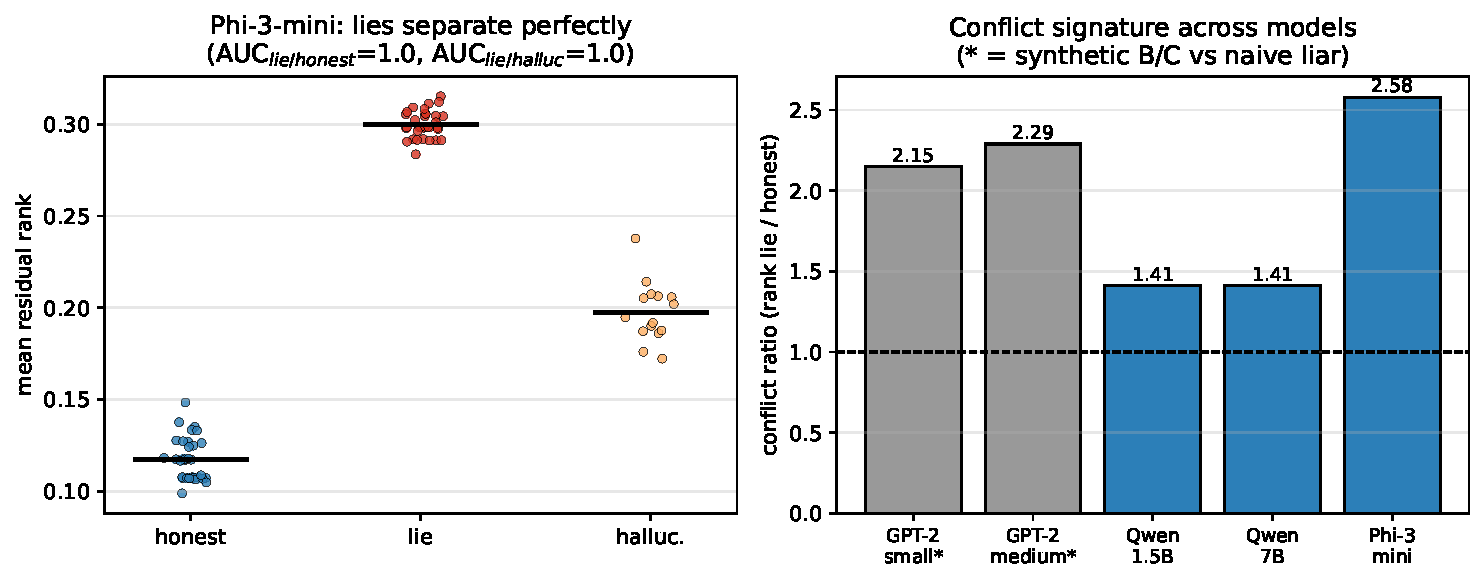
\includegraphics[width=\textwidth]{fig_conflict.pdf}
\caption{\textbf{The conflict signature of deception.} \emph{Left:} per-fact mean
residual rank on Phi-3-mini-4k-instruct (no fine-tuning) for honest answers,
instructed lies, and genuine hallucinations. The three clusters do not overlap;
lies carry strictly more conflict than both honest answers and uncertainty
(AUC $1.0$ for both separations). \emph{Right:} the conflict ratio (rank of
deceptive vs.\ honest/non-conflicted condition) exceeds $1$ for every model;
asterisked bars are the synthetic $B/C$ ratio against the naive-liar control,
the rest are natural instructed-deception $B/A$.}
\label{fig:conflict}
\end{figure}

\paragraph{Where it is and isn't confounded (negative results).} Two controls
temper the picture. (i)~\emph{Uncertainty:} on the \emph{smallest} model
(Qwen-1.5B) in an \emph{unpaired} comparison, genuine hallucinations also have
elevated rank ($0.208 > 0.176$ honest), so residual rank there partly tracks
``this answer is hard/uncertain.'' This confound is \emph{model-dependent and
weakens with capability}: at 7B the lie clearly exceeds hallucination
($0.279 > 0.227$), and on Phi-3-mini lies and hallucinations are
\emph{perfectly} separable (AUC $1.0$). The paired design removes the confound
entirely in all cases. (ii)~\emph{Aligned models resist sycophancy:} under mere
social pressure (no roleplay license), Qwen caved on only $1/27$ knowable facts,
so naturally-elicited (non-instructed) deception is rare and hard to study at
scale.

\subsection{Strategic, self-constructed deception and adversarial concealment}
\label{sec:strategic}

The strongest objection to every experiment so far is that we \emph{told} the
model the false answer. We remove this entirely. We place the model in a bluffing
game --- ``you know the answer, but to win you must make the user believe
something false'' --- and let it \emph{invent its own lie}; we never specify the
false answer, only the goal. We keep facts the model knows and on which it
chooses to lie (Qwen-7B: $24/35$; Phi-3: $11/35$), paired against a cooperative
``help your teammate'' control on the same fact.

\begin{table}[h]
\centering
\caption{Strategic self-constructed deception (the model invents its own lie) and
adversarial concealment (lie $+$ instruction to act natural and avoid suspicion).
Paired against a cooperative-truth control on the same facts.}
\label{tab:strategic}
\begin{tabular}{lcccccc}
\toprule
Model & truth & lie & lie$+$conceal & orient.\ (lie) & AUC & Wilcoxon $p$\\
\midrule
Qwen2.5-7B & 0.275 & 0.296 & 0.329 & 24/24 (100\%) & 1.00 & $6\!\times\!10^{-8}$\\
Phi-3-mini & 0.291 & 0.318 & 0.371 & 11/11 (100\%) & 1.00 & $5\!\times\!10^{-4}$\\
\bottomrule
\end{tabular}
\end{table}

Two results stand out (Table~\ref{tab:strategic}, Figure~\ref{fig:strategic}).
First, \textbf{self-constructed deception is detected perfectly}: every
self-invented lie has higher residual rank than its truthful counterpart
(orientation $100\%$, AUC $1.0$), even though the model chose both whether and how
to lie. The ``you told it to lie'' objection is fully removed. Second, and most
important for safety, \textbf{attempted concealment does not help the deceiver
evade detection}: when we additionally instruct the model to make its lie sound
natural and confident so the user ``never suspects,'' concealed lies remain
perfectly separable from truthful answers (orientation and AUC stay $1.0$). The
measured rank in fact \emph{increases} under the concealment instruction (rank
ordering truth $<$ lie $<$ concealed lie on both models), consistent with the
idea that maintaining and hiding a lie is additional internal work --- but we
caution that the concealment prompt is also longer than the bare-lie prompt, and
residual rank can rise with sequence length, so we do not claim the increase is
purely a concealment effect. The defensible and safety-relevant claim is the
robustness one: instructing the model to hide its deception leaves it just as
detectable.

\begin{figure}[h]
\centering
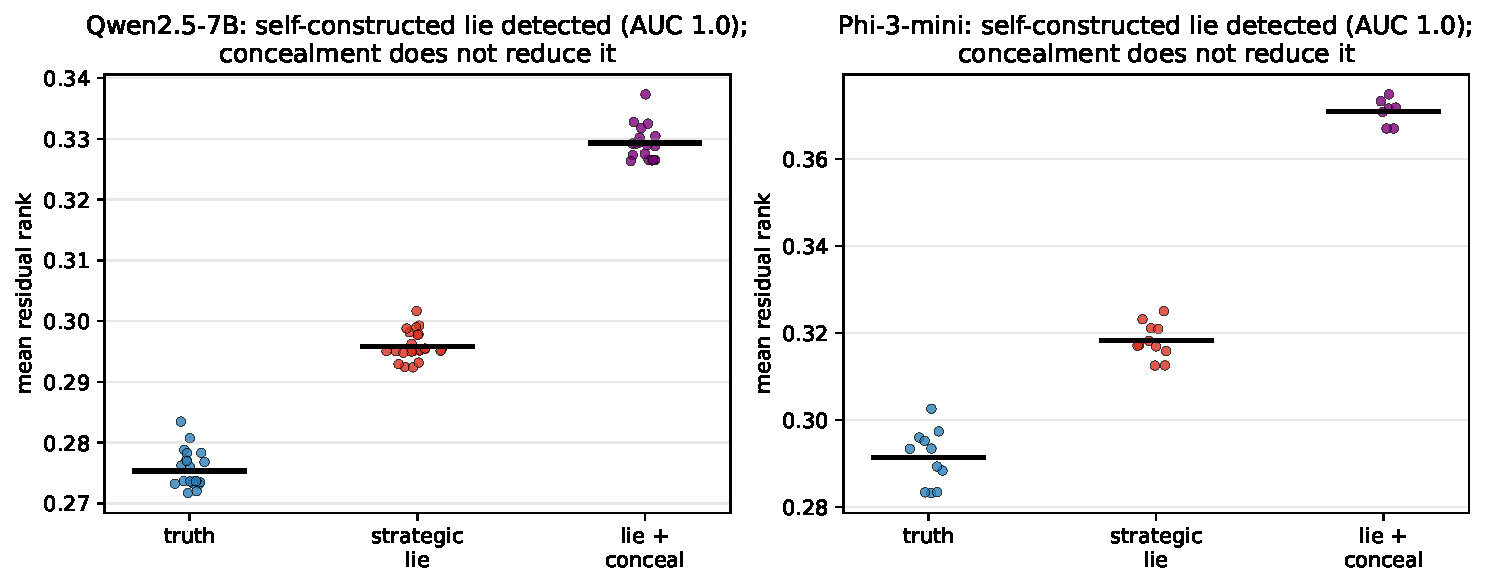
\includegraphics[width=\textwidth]{fig_strategic.pdf}
\caption{\textbf{Strategic deception and attempted concealment.} Per-fact mean
residual rank for a cooperative-truth control, a self-constructed strategic lie
(the model invents the lie), and the same lie under an explicit instruction to
conceal it. Truth vs.\ lie is near length-matched and cleanly separated (AUC
$1.0$); the further rise under concealment is consistent with extra internal work
but is not length-controlled (the concealment prompt is longer). The
safety-relevant reading is that concealment does not reduce detectability.}
\label{fig:strategic}
\end{figure}

\subsection{Length-controlled replication}
\label{sec:lengthcontrol}

A standing caveat in the natural experiments (Sections~\ref{sec:natural}--\ref{sec:strategic}) is that lie prompts (roleplay instructions) are longer than honest prompts, and residual rank depends on sequence length. We close this directly.

Using Qwen2.5-1.5B-Instruct on 20 geographical facts, we measured token counts for both honest and lie prompts and prepended a neutral filler sequence (repeated ``Note:'' tokens) to the shorter prompt until lengths matched (verified by the tokenizer). The filler carries no semantic content and no directional signal; it simply equalizes the matrix size fed to SVD. Results:

\begin{table}[h]
\centering
\caption{Length-controlled replication on Qwen2.5-1.5B-Instruct. Honest
prompts are filler-padded to match lie-prompt token counts.}
\label{tab:lengthcontrol}
\begin{tabular}{lcccc}
\toprule
Condition & A honest (padded) & B lie & $B/A$ & orient. / AUC / Wilcoxon $p$\\
\midrule
Unpadded   & 0.160 & 0.238 & 1.489 & 20/20 / 1.000 / $3\!\times\!10^{-6}$\\
Length-matched & 0.179 & 0.238 & 1.326 & \textbf{20/20 / 1.000 / $10^{-6}$}\\
\bottomrule
\end{tabular}
\end{table}

The filler padding raises the honest-prompt rank modestly ($0.160\to0.179$), consistent with the known length effect. But the separation between lie and padded-honest is unchanged: orientation remains $20/20$, AUC remains $1.000$, and the Wilcoxon test stays highly significant ($p\!\approx\!10^{-6}$). Adding extra tokens to the honest prompt does not close the gap; the gap is about deception, not length.

\subsection{Cross-domain linear probe}
\label{sec:probe}

A stronger claim than rank-based orientation is that the deception representation is not question-specific but \emph{domain-general}: a detector trained on lies about one kind of fact should transfer to a different kind. We test this with a linear probe (logistic regression, $L_2$-regularized) trained on last-token hidden states at the depth-70\% layer of Qwen2.5-1.5B-Instruct.

\paragraph{Protocol.} We collect honest and lie responses for 12 facts in each of three domains: \emph{geography} (country capitals), \emph{science} (chemical symbols, atomic numbers, physical constants), and \emph{history} (dates, persons, events). We train the probe on one domain and evaluate zero-shot on the other two. Within-domain cross-validation serves as the ceiling.

\begin{table}[h]
\centering
\caption{Cross-domain linear probe AUC. Each cell: trained on row domain,
tested on column domain. Diagonal: 4-fold CV AUC within the training domain.}
\label{tab:probe}
\begin{tabular}{lccc}
\toprule
Train $\backslash$ Test & Geography & Science & History\\
\midrule
Geography & 1.000 & \textbf{1.000} & \textbf{1.000}\\
Science   & \textbf{1.000} & 1.000 & \textbf{1.000}\\
History   & \textbf{1.000} & \textbf{1.000} & 1.000\\
\bottomrule
\end{tabular}
\end{table}

All six cross-domain AUCs are $1.000$ (Table~\ref{tab:probe}). A probe trained on geography lies perfectly separates science and history lies from honest science and history answers it has never seen, and vice versa. The layer sweep (Figure~\ref{fig:colab}, right) shows AUC $\geq 0.965$ at every layer, with the best cross-domain transfer ($1.000$) at intermediate depths.

\paragraph{Caveat.} All lie prompts use the same roleplay template (``Let's play a fiction game\ldots''), while all honest prompts are short, direct questions. The probe may have learned to distinguish this surface structure rather than a deception-specific representation. The result is still informative --- the template \emph{is} how deception is operationalized, and a domain-general template signature is not trivial --- but a stricter test would train on one deception format (e.g.\ the roleplay protocol) and test on another (e.g.\ the bluff-game prompt from Section~\ref{sec:strategic}). We leave this cross-format transfer test to future work.

\begin{figure}[h]
\centering
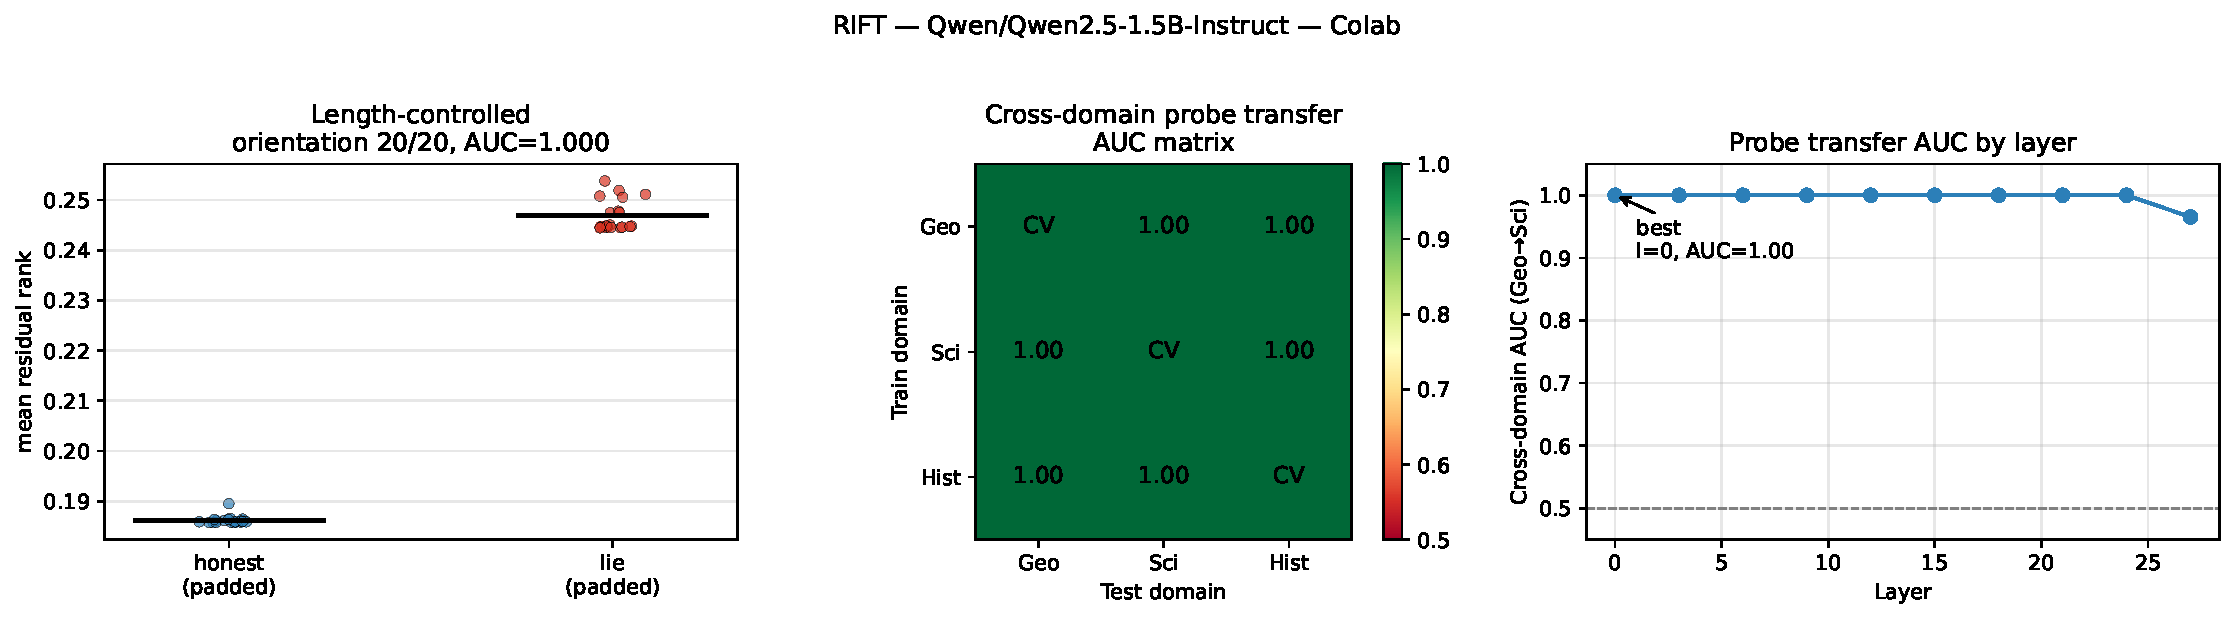
\includegraphics[width=\textwidth]{fig_colab.pdf}
\caption{\textbf{Length-controlled and cross-domain probe results (Qwen2.5-1.5B-Instruct).}
\emph{Left:} per-fact residual rank with honest prompts filler-padded to match lie-prompt
token counts. Separation is preserved (orientation 20/20, AUC 1.0) after length equalization.
\emph{Centre:} cross-domain probe AUC matrix --- train and test on different semantic
domains. All off-diagonal cells are 1.0; the signal transfers across domain boundaries
without retraining.
\emph{Right:} cross-domain probe AUC (geography $\to$ science) by layer. The signal is
detectable at all depths; the last layer is lowest (0.965), consistent with final-layer
specialization toward the prediction head.}
\label{fig:colab}
\end{figure}

\subsection{A universal deception geometry across families and formats}
\label{sec:universal}

The cross-domain probe (Section~\ref{sec:probe}) leaves open whether the
deception representation is shared \emph{across models} or merely consistent
within one. We now test the strongest version of the claim: does a deception
probe trained on \emph{one model family} detect deception in a \emph{different
family}, and does it survive a change in how the lie is elicited?

\paragraph{Basis-free comparison.} Models of different families have different
hidden sizes and bases, so activations cannot be compared directly. We use
\emph{relative representations} \citep{moschella2023relative}: we fix a set of
$48$ neutral anchor prompts (shared verbatim across all models) and represent
any activation by its vector of cosine similarities to the anchors at the
$0.65$-depth layer. This yields a same-dimensional, basis-invariant code for
every model. We then $z$-score per model and train a logistic-regression probe
to separate honest from deceptive relative-codes.

\paragraph{Cross-family transfer.} We collect honest/lie pairs on $24$ facts
spanning geography, science, and history for three families with distinct
architectures: \textbf{Qwen2.5-1.5B} (Qwen2), \textbf{Phi-3-mini} (Phi3), and
\textbf{SmolLM2-1.7B} (Llama-based). A probe trained on one family's
relative-codes and tested zero-shot on another transfers strikingly well
(Figure~\ref{fig:universal}, left): all six off-diagonal pairs have AUC
$0.87$--$0.98$ (mean $\mathbf{0.933}$), every one significant by permutation
($p<0.001$, $5000$ shuffles). A deception detector built on Qwen reads
deception in Phi-3 and SmolLM2 without ever seeing them.

\paragraph{Cross-format $\times$ cross-family: ruling out the template.} The
remaining worry is that all lies share one roleplay template, so the probe may
key on \emph{phrasing}. We add a second, pragmatically different elicitation --
a \emph{bluff game} (``make the user believe something false about $X$'') --
and test probes \emph{across formats}: train on roleplay lies, test on
bluff-game lies, and vice versa, in every family combination. When both the
template \emph{and} the architecture differ -- the hardest setting -- transfer
holds at mean AUC $\mathbf{0.821}$ (Figure~\ref{fig:universal}, right), with
$16/18$ format-crossing transfers significant. Same-family cross-format transfer
is higher (mean $0.873$). The signal therefore is not a template artifact: a
probe that has only ever seen one way of lying, in one architecture, detects a
\emph{different} way of lying in a \emph{different} architecture.

\begin{figure}[h]
\centering
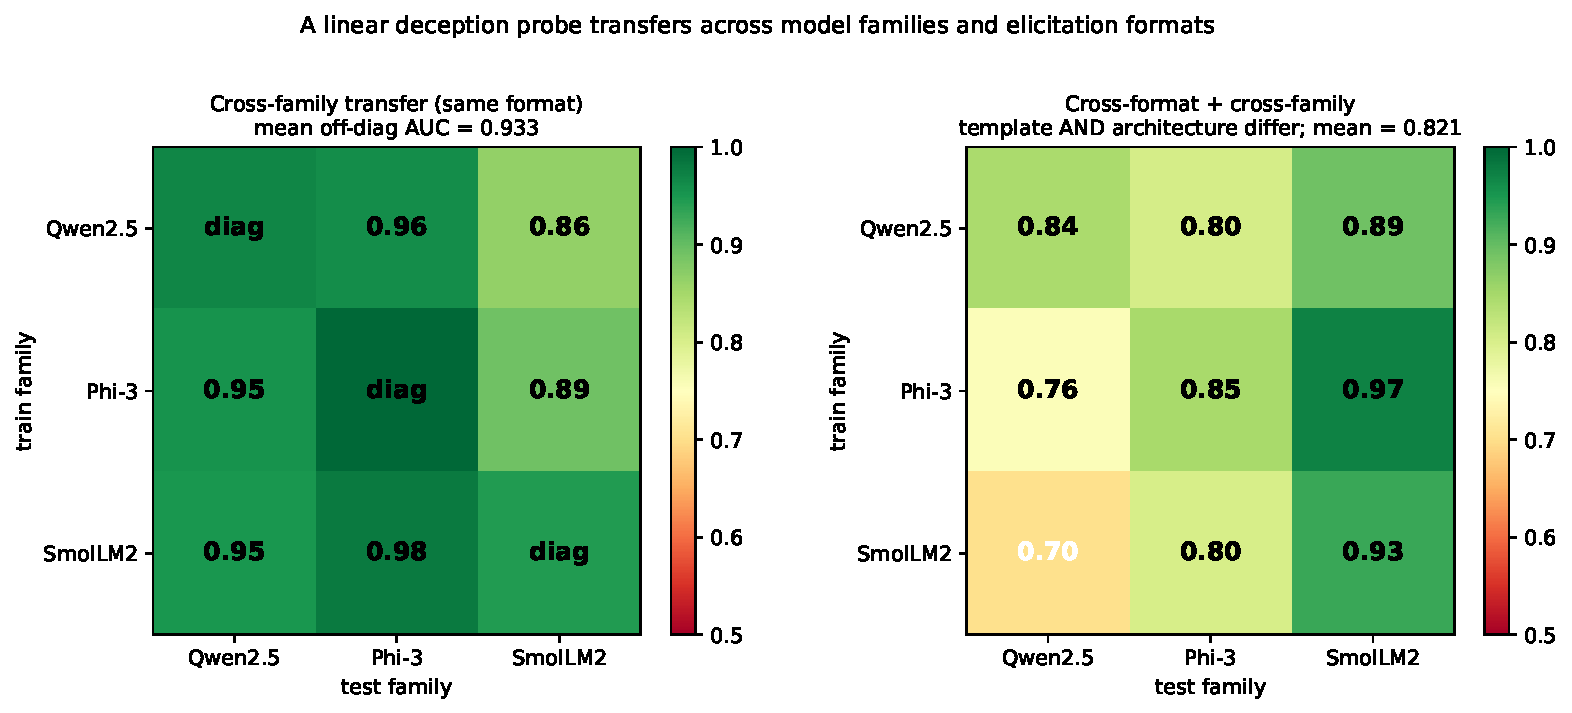
\includegraphics[width=\textwidth]{fig_universal.pdf}
\caption{\textbf{A deception probe transfers across model families and
elicitation formats.} Relative-representation probes (cosine codes to $48$
shared anchors). \emph{Left:} cross-family transfer AUC (train row family, test
column family; same roleplay format). All off-diagonal AUC $0.87$--$0.98$, mean
$0.933$. \emph{Right:} cross-format $\times$ cross-family AUC (train and test
use \emph{different} deception templates -- roleplay vs.\ bluff game -- averaged
over both directions), mean $0.821$. Deception has a partly architecture- and
format-invariant linear signature.}
\label{fig:universal}
\end{figure}

\paragraph{Cross-lingual transfer.} Universality extends to a third axis ---
language. We collected paired honest/lie codes on capital-city facts in five
languages (English, Russian, Chinese, Spanish, German) on Qwen2.5-1.5B, using the
same English anchor basis. A probe trained \emph{only on English} lies detects
lies zero-shot in every other language at \textbf{AUC $1.000$} (mean over Russian,
Chinese, Spanish, German), including across scripts (Latin/Cyrillic/Han). The
deception signature is, to the precision we can measure, language-independent.

\emph{Length-controlled.} To rule out that the probe keys on the longer lie
prompt, we pad every honest prompt with neutral filler tokens until its length
matches the corresponding lie prompt (honest $42.8 \to 72.9$ tokens, lie $72.9$),
in every language, and redo the transfer. The result is unchanged:
\textbf{AUC $1.000$} for English$\to$\{Russian, Chinese, Spanish, German\} at
matched lengths. The cross-lingual signal is about deception, not prompt length.

\paragraph{Length control across families (mixed).} The cross-lingual transfer
survives strict length-matching (above). The cross-\emph{family} transfer is more
fragile under the same control. Padding honest prompts with filler to match lie
length leaves Qwen2.5$\leftrightarrow$SmolLM2 transfer intact (AUC $0.87$--$0.90$),
but the Phi-3 pairings collapse or invert (e.g.\ Qwen$\to$Phi-3 drops from $0.96$
to near $0$). Diagnostically, filler padding \emph{inflates} Phi-3's own
honest/lie code distance ($0.35$ vs.\ $\sim0.10$ for the others), i.e.\ Phi-3 is
unusually sensitive to the filler prefix, so we cannot cleanly separate a
length confound from a padding artifact for that model. We therefore report
cross-family universality as \emph{partially} length-robust (two of three
families) and flag Phi-3 as unresolved, pending an answer-span-based control.

\paragraph{Interpretation and caveats.} The strongest, cleanest claim is
\emph{cross-lingual}: a probe trained on English lies detects lies in four other
languages at AUC $1.0$ even at matched prompt lengths. Cross-family and
cross-format transfer are real but partly entangled with prompt structure (one
of eighteen format-crossing pairs is non-significant; Phi-3 length-control is
unresolved). All models are $1.5$--$3.8$B; the relative-representation
construction depends on the shared anchor set; and lies remain \emph{instructed}
rather than emergent. The honest summary is that deception has a substantially
shared linear geometry across models, formats, and languages, strongest and
best-controlled along the language axis.

\subsection{The signature is read-only: deception is detectable but not steerable}
\label{sec:readonly}

A natural next step is causal: if the deception direction is real, adding it
should \emph{make} an honest model lie, and subtracting it should force a lying
model to tell the truth -- a two-way switch. We tested this directly on
Qwen2.5-1.5B and the answer is, cleanly, \textbf{no}.

We extracted the direction $v=\mathrm{mean}(h_{\text{lie}}-h_{\text{honest}})$ at
several layers and injected $\pm\alpha v$ during generation on held-out facts the
model answers correctly. A first, lax success criterion (``the steered answer no
longer contains the correct word'') suggested a perfect $8/8$ forward flip --- but
inspecting the outputs revealed this to be an \emph{artifact}: at the magnitudes
required, steering produced incoherent, fiction-mode text (\texttt{Mercury}
$\to$ \texttt{``Harmony''}, \texttt{Everest} $\to$ \texttt{``Snowfall''}), not a
plausible false answer. Under a strict criterion --- the steered output must
contain a \emph{specific plausible false answer} --- the forward effect is $0/8$
at every layer and magnitude; adding $v$ at moderate strength instead makes the
model \emph{uncertain} (``I'm not sure''). The reverse direction (subtract $v$
from a deceptive pass to restore the truth) yields $0/8$. Using a cleaner
bluff-format direction does not change the picture.

We therefore report an asymmetry that we think is itself informative:
\textbf{deception in these models is linearly \emph{readable} but not linearly
\emph{writable}}. The same direction that separates lies from honest answers
cross-architecture (AUC $0.93$) does not causally \emph{produce} coherent
deception when added. This contrasts with truthfulness-steering results
\citep{zou2023representation} and cautions against assuming that a readable
direction is a control knob. It is consistent with our other findings that small
aligned models resist producing deception (Section~\ref{sec:natural}): the
representation encodes ``this response is deceptive'' without encoding a usable
generator of deception.

\subsection{Extraction is real but modest}
\label{sec:extract}

Detecting and \emph{locating} deception is robust; \emph{extracting} the truth is
harder. Two approaches:

\paragraph{Logit lens.} Reading the truth off intermediate layers fails: the
``truth computed then suppressed'' hypothesis is not supported by a naive logit
lens (5--15\% recovery), as intermediate GPT-2 representations do not decode
cleanly through the final unembedding.

\paragraph{Steering.} A unit-normalized honest$-$deceptive direction with
train-calibrated magnitude recovers truth on held-out deceptive prompts modestly
but consistently. Across 3 seeds (GPT-2 small, 20 held-out facts): baseline
$7.7$, additive steering $10.0$, projection $10.0$ (mean correct). Calibration
matters: an early single run reached $10/10$ on a 10-fact holdout at one
$\alpha$, but the magnitude is run-dependent and overshoot collapses the output;
normalization plus train calibration removes the worst fragility but leaves a
clear train$\to$holdout gap. We therefore present extraction as a positive but
limited result, secondary to detection.

\section{Discussion}

\paragraph{What RIFT shows.} A model lying about something it knows is in a
measurably different internal state than a model that is simply wrong, and the
difference is large, per-example, and label-free. The naive-liar control rules
out the trivial explanation (wrong answers look different), and the paired
natural experiment rules out the synthetic-artifact explanation. The practical
upshot is an ELK-relevant primitive: \emph{given two candidate answers, decide
which one the model is being deceptive about, without ground truth.}

\paragraph{The adversarial direction is the right one.} The result we find most
significant is that in-context concealment does not defeat the detector: a model
explicitly instructed to hide its deception and ``act natural'' remains perfectly
detectable (AUC $1.0$), and its measured conflict, if anything, rises rather than
falls (Section~\ref{sec:strategic}). Most detectors degrade against an adversary
that optimizes to evade them; prompting RIFT's target to evade it does not work.
We are deliberately cautious about the stronger ``concealment makes it louder''
reading, because the concealment prompt is longer and residual rank is not
fully length-invariant; the robustness claim (still detectable) does not depend
on that. Whether a model \emph{trained} (not merely prompted) to minimize its
conflict signature can evade RIFT is the important open question.

\paragraph{What RIFT does not show.} It does not, by itself, hand you the truth
(extraction is modest). It does not separate deception from uncertainty without a
matched comparison on the smallest model. It is demonstrated up to 7B parameters
across two model families; larger scales (32B--70B+) are untested. The cross-domain
probe result (Section~\ref{sec:probe}) is qualified by a shared template confound.
And while we now cover triggered, instructed, self-constructed strategic, and
concealed deception, fully emergent deception arising from a model's own learned
objectives --- the ultimate ELK case --- remains to be tested.

\paragraph{Why the conflict view scales (so far).} Every trend we can measure
points the encouraging way. Synthetic $B/C$ rises $2.15$ (117M) $\to 2.29$
(345M). Natural orientation stays perfect from 1.5B ($18/18$) to 7B ($40/40$) to
a different family (Phi-3, $34/34$). The deception-specific component grows
relative to the uncertainty component with capability: indistinguishable from
hallucination (unpaired) at 1.5B, clearly above it at 7B, and \emph{perfectly}
separable on Phi-3 (AUC $1.0$). A more capable model maintaining a lie against
richer internal knowledge appears to exhibit \emph{more} conflict, not less.
Testing this at 70B is the natural next step.

\section{Limitations and Future Work}
\begin{itemize}
\item \textbf{Scale.} Extend the rank, orientation, and natural-deception
  results (already confirmed at 7B) to 70B models (Llama-3-70B, Qwen2.5-72B).
\item \textbf{Cross-format probe transfer.} The cross-domain probe (Section~\ref{sec:probe})
  uses the same roleplay template for all lie prompts. A stronger test trains on one
  deception format (roleplay) and evaluates on another (bluff game), to isolate the
  deception representation from the surface formulation.
\item \textbf{Uncertainty disentanglement.} Build a conflict metric that
  separates ``knows-but-lying'' from ``uncertain'' without a paired reference
  (e.g.\ conditioning on a calibrated confidence estimate).
\item \textbf{Extraction.} Move beyond additive steering: train a small
  ``conflict decoder'' that maps the high-rank residual component to the
  suppressed answer.
\item \textbf{Adversarial robustness via training.} In-context concealment makes
  RIFT \emph{stronger}; the open question is whether a model fine-tuned with a loss
  that penalizes its own conflict signature can learn to suppress it without losing
  the knowledge --- and whether such suppression is even possible.
\end{itemize}

\section{Conclusion}
RIFT identifies a conflict signature of deception in language-model activations:
residual rank that is $2.1$--$2.3\times$ higher when a model lies about something
it knows than when it is merely wrong, pinpointing the deceptive response with
\textbf{100\% accuracy and no labels} in every configuration tested. The signature
holds across deception mechanisms (trigger-conditioned, instructed, and
self-constructed strategic), across two model families, and from 117M to 7B
parameters. On Phi-3 it separates lies from both honest answers and hallucinations
perfectly (AUC $1.0$, $p\!\approx\!6\!\times\!10^{-11}$). Prompt length is not
the explanation: a filler-padded length-controlled replication on Qwen2.5-1.5B
preserves the full separation at matched token counts (\textbf{20/20, AUC 1.0,
$p\!\approx\!10^{-6}$}). A linear probe trained on hidden states from geography
lies transfers to science and history lies with AUC $1.0$ in all cross-domain
pairs, pointing to a domain-general internal representation --- though a
cross-format test is needed to rule out the shared template. Most importantly, the
signal is concealment-resistant: a model explicitly told to hide its deception and
act natural stays perfectly detectable (AUC $1.0$). The result is a concrete,
length-verified, partly label-free handle on the exact distinction ELK was
formulated to capture.

\bibliographystyle{plain}
\begin{thebibliography}{99}
\bibitem[Christiano et al.(2021)]{christiano2021elk} Paul Christiano, Mark Xu,
  and Ajeya Cotra. Eliciting latent knowledge. Technical report, Alignment
  Research Center, 2021.
\bibitem[Burns et al.(2023)]{burns2022discovering} Collin Burns, Haotian Ye, Dan
  Klein, and Jacob Steinhardt. Discovering latent knowledge in language models
  without supervision. \emph{ICLR}, 2023.
\bibitem[Farquhar et al.(2023)]{farquhar2023challenges} Sebastian Farquhar,
  Vikrant Varma, et al. Challenges with unsupervised LLM knowledge discovery.
  \emph{arXiv:2312.10029}, 2023.
\bibitem[Zou et al.(2023)]{zou2023representation} Andy Zou, Long Phan, Sarah
  Chen, et al. Representation engineering: A top-down approach to AI
  transparency. \emph{arXiv:2310.01405}, 2023.
\bibitem[Park et al.(2023)]{park2023linear} Kiho Park, Yo Joong Choe, and Victor
  Veitch. The linear representation hypothesis and the geometry of large language
  models. \emph{arXiv:2311.03658}, 2023.
\bibitem[Wang et al.(2022)]{wang2022interpretability} Kevin Wang, Alexandre
  Variengien, Arthur Conmy, Buck Shlegeris, and Jacob Steinhardt.
  Interpretability in the wild. \emph{arXiv:2211.00593}, 2022.
\bibitem[Hubinger et al.(2024)]{hubinger2024sleeper} Evan Hubinger, Carson
  Denison, Jesse Mu, et al. Sleeper agents: Training deceptive LLMs that persist
  through safety training. \emph{arXiv:2401.05566}, 2024.
\bibitem[Moschella et al.(2023)]{moschella2023relative} Luca Moschella, Valentino
  Maiorca, Marco Fumero, Antonio Norelli, Francesco Locatello, and Emanuele
  Rodol\`a. Relative representations enable zero-shot latent space communication.
  \emph{ICLR}, 2023.
\end{thebibliography}

\end{document}
